\chapter{Introduction} \label{sectionIntroduction}

\todo{TODO: Chapter 1 - introduction into what I did}

When building software systems, we have several areas of concern: cost, delivery timeline, quality, etc. The cost and time-to-market are often the two problems given the highest priority in a project. However, engineers must consider the software quality to preserve the system's longevity. Despite its importance, the code and architecture quality can be challenging to understand and measure.

When we think about projects, we can assume that as time goes on and changes and additions occur within a system's source code, the complexity of that system will grow (``Fig.~\ref{figTimeAndComplexity}''). However, when we manage the code structure, we can keep the complexity in check, allowing systems to evolve. Developers can maintain this structure through simple steps like having readable code and more complex considerations, like how coupled and cohesive a system is.

\begin{wrapfigure}{r}{0.5\textwidth}
    \centering
    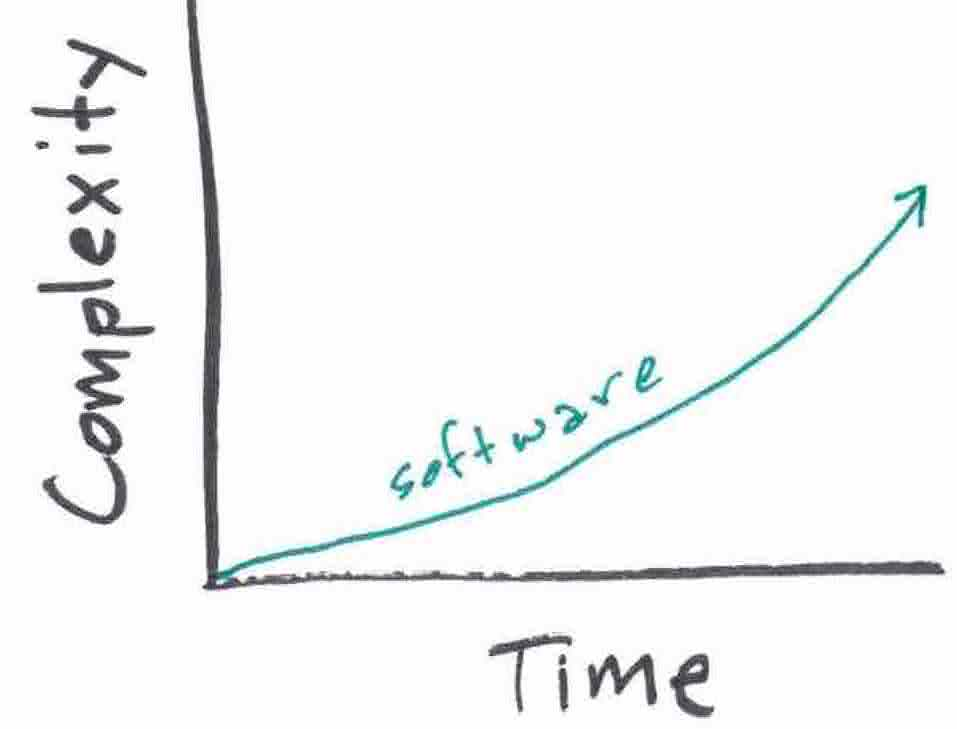
\includegraphics[width=0.5\textwidth]{TimeAndComplexity}
    \caption{Generally speaking, a software system will get more complex as it grows over time.}
    \label{figTimeAndComplexity}
\end{wrapfigure}

One way to understand the quality around a system is to discuss its ``maintainability,'' the ease of receiving new features or resolving bugs. For example, developers may find that adjusting one area to add a new feature requires touching several other code areas in tightly coupled systems. Some code measuring systems provide a Maintainability Index, a well-known quality measure. However, its effectiveness in quantifying software quality is debated \cite{vandeursen:2014}.

On the other hand, code smells are used extensively by practitioners to identify low-quality spots in the software system. These areas would need the teams' attention and are good candidates for refactoring.

Pylint is a static analysis tool that identifies several classes of code quality concerns, particularly relevant to our study, refactor violations, which report on various code smells. We can assume that there must be some correlation between Maintainability Index and the type and number of code smells in a software system, quantified by the Pylint refactor score.

This study explores such assumptions and systematically investigates any correlation between the Maintainability Index metric and the Pylint Refactor score. Furthermore, we perform analysis on specific refactor violations to reveal and shed light on the relative effectiveness of the different refactor violations and their relationship to Maintainability Index.

The structural quality of a software system will impact the software evolution. If the project has poor structural quality, the architecture will minimize its ability to evolve, and the software system will eventually ``die-off'' so to speak.

Why should we care about whether the code is maintainable? It is assumed that a large amount of the cost over the lifetime of a project is attributed to maintainability. Fred Brooks, in his book ``The Mythical Man-Month'' even claimed that over 90\% of the costs for a typical software system come up in the maintenance phase \cite{brooks:mythical}. Once the bulk of the system is off the ground and live worldwide, how well the team can improve the system with new features and fix bugs, even working on different parts in parallel, can be impacted by its maintainability. Any successful piece of software will inevitably need to be maintained.

We will look at many open-source Python systems using Pylint and attempt to correlate the data from the Pylint scores to the level of ease in adding new features to the system. This will determine if a system is more maintainable with better Pylint scores. 

\todo{TODO: Conclude with a summary of the organization of the thesis, including identification of the general content of specific chapters and appendices.}

% --- SUMMARY OF CONTRIBUTIONS ------------------------------------------------
% --- How does my idea solve the problem? -------------------------------------
% --- THE PROBLEM: Some projects fail to evolve, resulting in loss if income.
% --- MY IDEA: Software evolution is impacted by structural quality.
% -----------------------------------------------------------------------------

We will explore automated measurements that provide evaluation scores of software systems. By using some of these quality and maintainability scores, we can see how structure impacts evolution (Section \ref{sectionMyIdea}). In our case, we will explore the Pylint Refactor score on commits for new features, focusing specifically on the adaptability and evolution of a software project (Sections \ref{sectionSoftwareData} and \ref{sectionMaintainabilityScores}).

When a team is able to embrace and use these types of measurements from the beginning of a project, it enables faster architecture review than checking it only by hand. These types of measurements can inform us of areas with ``smells,'' providing insight on where to focus on improvements. In addition to the usefulness at the beginning of a project, continuing to revisit these numbers on a regular basis (every sprint, for example, in a scrum team) keeps the project in a maintainable state.

% \todo{TODO: what is the specific, refutable information that we found?}

In addition to using scores to predict software evolution ability, we also look at documentation used in the best and worst projects to determine that good documentation can improve maintainability (Section \ref{sectionDocumentation}).

\todo{TODO: Update sections listed above?}
